
\documentclass{sig-alternate}



%\usepackage{cite}
%\usepackage{graphicx}
%\usepackage{hyperref}
%\usepackage{listings}
%\usepackage{times}
%\usepackage{xspace}
%\usepackage{subfigure}
%\usepackage{fancybox}
%\usepackage{multirow}
%\usepackage{array}
%\usepackage{subfigure}
%\usepackage{balance}
%\usepackage{tabularx}
%\usepackage{url}
%\usepackage{listings}
\usepackage{booktabs}
\usepackage{color}


\newcommand{\todo}[1]{\textcolor{cyan}{\textbf{[#1]}}}
\newcommand{\emad}[1]{\textcolor{red}{{\it [Emad says: #1]}}}
\newcommand{\dan}[1]{\textcolor{blue}{{\it [Dan says: #1]}}}
\newcommand{\sam}[1]{\textcolor{green}{{\it [Sam says: #1]}}}
\newcommand{\feedback}[1]{\textcolor{green}{{\it [Feedback says: #1]}}}




\begin{document}
%
% --- Author Metadata here ---
\conferenceinfo{ICSE}{'14 Hyderabad, India}
%\CopyrightYear{2007} % Allows default copyright year (20XX) to be over-ridden - IF NEED BE.
%\crdata{0-12345-67-8/90/01}  % Allows default copyright data (0-89791-88-6/97/05) to be over-ridden - IF NEED BE.
% --- End of Author Metadata ---

\title{Concolic Analysis for Code Clone Detection} % Work on this title

\numberofauthors{1} %  in this sample file, there are a *total*
% of EIGHT authors. SIX appear on the 'first-page' (for formatting
% reasons) and the remaining two appear in the \additionalauthors section.
%
\author{
%
% 1st. author
\alignauthor
Daniel E. Krutz,  Emad Shihab, and Samuel A. Malachowsky\\ 	
	\affaddr{Software Engineering Department}\\
       \affaddr{Rochester Institute of Technology, USA}\\
     %  \affaddr{1 Lomb Memorial Drive}\\
   %    \affaddr{Rochester, NY } \\
       \email{\{dxkvse, emad.shihab, samvse\}@rit.edu}
} % Must not be a space above this

\maketitle



% This abstract does not look like it is properly formatted
\begin{abstract}

Source code is often duplicated throughout software projects. These duplicated functionality equivalent portions of an application are known as code clones. Clones may be problematic for several reasons, some of which include elevated maintenance costs and increased system faults. While there are a wide range of powerful techniques for finding these clones, most struggle at detecting the most complicated types of code clones, type-4 clones. In this work, we propose a new type of clone detection technique, which uses concolic analysis. Through a case study, we demonstrate the effectiveness of concolic analysis in clone discovery and its ability at identifying type-4 clones. We discuss our preliminary results and describe the future work we plan on conducting.

% Did we already demonstrate the effectivness in the WCRE paper?
% I think this ending sounds kind of weak.
% The abstract could be longer.
% Really work on it.


\end{abstract}

% A category with the (minimum) three required fields
%\category{H.4}{Information Systems Applications}{Miscellaneous}
%A category including the fourth, optional field follows...
%\category{D.2.8}{Software Engineering}{Metrics}[complexity measures, performance measures]

%\terms{Theory}

%\keywords{ACM proceedings, \LaTeX, text tagging}



\section{Introduction}

% Make sure this is significantly different than the tools paper
Research has shown that between 7\% and 23\% of a software system is comprised of clones~\cite{Roy:2008:ESF:1447565.1448036}~\cite{Baker:1995:FDN:832303.836911}. This is likely very problematic since clones, and their inconsistent maintenance, have been shown to widely lead to a high level of system faults~\cite{Juergens:2009:CCM:1555001.1555062}. Clones also increase the maintenance costs of an application since the same alteration may need to be done multiple times in all of the cloned elements~\cite{Li:2006:CFC:1128600.1128814}. While there are four types of code clones, only two known techniques state that they are able to reliably detect type-4 clones. These clones are typically the most difficult to detect and may be much more problematic than the simpler types of clones~\cite{Yuan:2011:CCM:2114489.2114766}~\cite{Roy07asurvey}.

% Is it ok to discuss all four types of clones here, but introduce them later? % yes it is fine.


% How to best reference this work? And is this the place to do it.
In a previous work, we created a clone detection tool based upon concolic analysis, called Concolic Code Clone Detection (CCCD)~\cite{wcre2013}. This tool demonstrated the effectiveness of concolic analysis in discovering clones in a small, controlled environment. 

In this paper, we propose using concolic analysis to discover clones. This research is innovative because to our knowledge, no previous attempts have been made in using concolic analysis in clone discovery and any techniques which can effectively discover all four types of code clones are important since so few clone detection processes are able to do so. We want to present our early findings using concolic analysis for clone discovery and demonstrate our plan for future work. \emad{We do not say what is new over the tools paper here.}



\subsection{Code Clones}

There are four types of code clones which are generally recognized by the research community. Type-1 clones are the simplest types of clones and represent identical code except for variations in whitespace, comments and layout~\cite{4288192}. Type-2 clones contain variations in identifier types, but are otherwise syntactically similar. Type-3 clones contain altered or removed statements between two functionally equivalent code segments. Type-4 clones are two segments which are considerably different syntactically, but produce identical results when executed. Type-4 clones also represent the most difficult type of clone to detect~\cite{Gold:2010:ICC:1808901.1808916}~\cite{Dang:2012:XTC:2420950.2421004}.

Code clones are usually viewed as being problematic for several reasons. Clones will likely elevate maintenance efforts since bug fixes and code adaptation may need to be done multiple times, along with the need for extra testing and verification activities. Program comprehension, code quality analysis and aspect mining efforts  may also be increased due to the existence of code clones. Other uses for clone detection techniques include plagiarism analysis, software evolution analysis and virus detection~\cite{Roy:2009:CEC:1530898.1531101}.

% Other possible topics include
	% Why do developers create clones?
	% Not all clones are bad.
	% Show examples of clones here?


\subsection{Concolic Analysis}

Concolic analysis combines concrete and symbolic values in order to traverse all possible paths of an application (up to a given length). Concolic analysis is a variation of symbolic analysis were concrete executions are simultaneously run with symbolic analysis. In order to examine application paths, solvers are generated which are used to generate new test input to direct the application along the various execution paths. This process is continued until all possible distinct paths have been reached using a depth search strategy~\cite{Sen:2005:CCU:1081706.1081750}. The use of concrete values represents the primary advantage of using concolic analysis instead of symbolic analysis since constraints may be simplified which may assist in the precise reasoning of complex data structures. Concolic analysis has been traditionally used for testing due to its ability to traverse a large number of application paths~\cite{Majumdar:2007:HCT:1248820.1248874}. \emad{This paragraph sounds similar to the tools paper. Are you sure it is different?}







% Waiting until paper is better organized to write this section
%The remainder of this paper is organized as follows. Section~\ref{sec: whyconcolicworks} describes why 



\section{Detecting Clones Using Concolic Analsysis} 
\label{sec: howconcolicworks}

% Really work on making sure this section is understandable

The initial step is to perform concolic analysis on the chosen application. This may be accomplished through the use of several existing concolic analysis tools such as CREST~\footnote{http://code.google.com/p/crest/}, Java Path Finder (JPF)~\footnote{http://babelfish.arc.nasa.gov/trac/jpf/}, or CATG~\footnote{https://github.com/ksen007/janala2}. The generated concolic output is then separated at the method level, and then compared to other concolic method output in a round robin fashion so that all methods are compared to one another. Figure~\ref{fig:cccdstructure} presents the basic structure of CCCD.
% Should I describe this more?

\dan{Did I do a good enough job describing the concolic analysis process?}
\emad{I feel like you need a little more of a description here.}

\begin{figure}[thb!]
\vspace{2mm}
\centering
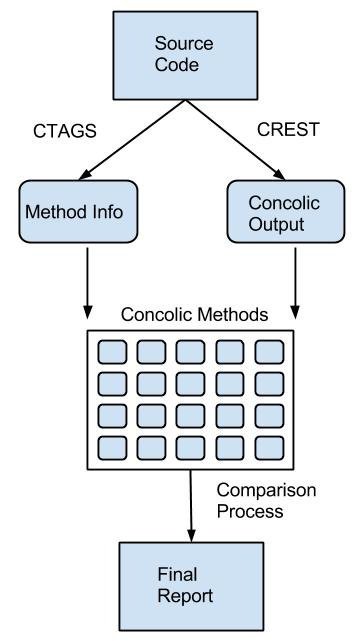
\includegraphics[width=33mm,height=60mm]{images/CCCDStructure_2.jpg}
\caption{Overview of the CCCD Tool~\cite{wcre2013}}
\label{fig:cccdstructure} % Label here is correct according to ICSE website
\end{figure}



% In our analysis using these tools, no special configuration was required 
%Discuss the trials done above? Should I mention how we have done testing with both Crest and JPF?

The Levenshtein distance algorithm \emad{Levenshtein is a distance metric, not algorithm. Or is it?} is used to evaluate the similarity of two sets of compared concolic output. We chose to use the Levenshtein algorithm to measure the similarity of the concolic output because of its ability to work with strings of different lengths and its restriction of upper and lower bounds in the calculated distances. In order to assist in normalizing the differences for strings of different lengths, the final calculated Average Levenshtein Value (ALV) is calculated by dividing the Levenshtein distance between the two compared methods (LD) by the longer of the two strings being compared (LSL) and then multiplying this value by 100. This formula is demonstrated in Equation~\ref{eq:avglevenformula}. For our initial work, we chose to state that any two compared methods with a Levenshtein distance of 30 or less would be considered a clone. However, this value may be altered in future use. \emad{Also, this seems very familiar from the tools paper. Ot am I just on crack?}

\begin{equation} \label{eq:avglevenformula}
ALV = (LD/LSL) \times 100
\end{equation}

Concolic analysis forms the basis of a powerful clone detection system because it only considers the functional paths of the examined source code. Similar functional paths represent a code clone candidate. Things such as comments, spacing and naming conventions with have been problematic for existing clone detection techniques have little effect on the ability of concolic analysis to detect clones. Since these items are irreverent, the amount of normalization which must be done using concolic analysis is minimal, especially when compared with many clone detection tools such as CCFinder and NICAD~\cite{Roy:2009:CEC:1530898.1531101}.


% This is really a problem with our implementation, not of concolic analysis for clone detection.

Our proposed technique does have two significant deficiencies. While future work may be done to mitigate this issue, our proposed method will only discover clones at the method level since this is where the concolic output is divided. This means that our technique will not discover a large number of clones that occur at a more granular level. Secondly, like all techniques, concolic analysis is not capable of discovering all types of clones in all situations. There are a large number of scenarios where concolic analysis will not discover clones. We do not believe this is an overly problematic issue for concolic analysis since all clone detection techniques suffer from this issue.


% Should we also state that we may examine the use of other distance measurement algorithms? %emad: sure!

% Discuss how concolic analysis may be done for each method. We use the default settings for the tool. The concolic application will handle all inputs and outputs automatically with us doing little to no work.




% Is the ordering and flow of this section correct? I feel like it is a bit choppy
% Should I describe the Levenstein formula any more than I do?
% Really discuss WHY it works.

\section{Case Study Results}

% Introduction to case study? - Describe the 3 aspects
In order to demonstrate the capability of concolic analysis for discovering code clones, we conducted an initial assessment using a self-created oracle. We then ran concolic analysis against this oracle recording types of clones discovered, false positives and false negatives. 



\subsection{Data}

The initial phase of our case study was to select several open source applications to examine for code clones. We chose to examine Apache 2.2.14, Python 2.5.1 and PostgreSQL 8.5 since they have already been used in previous clone detection research~\cite{Kim:2011:MMC:1985793.1985835}. These applications were selected as-is and had no alterations performed on their source code.
\dan{I feel like this section is a bit weak}


% Describe the data here

\subsection{Clone Oracle}

The first step was to identify existing clones in these systems. In order to make this process more manageable, we chose to analyze a small, statistically significant, subset of each application selecting several random class to examine. Even though only a small subset of each application was analyzed, since every method would be compared against each other, this made the number of possible clones to check for exponentially large. For the three applications, there were a total of 45,109 possible clones to check for, which was not reasonable to inspect through manual analysis.\dan{Actually, more were examined due to how each application had a stat sig value selected from them} To make this number more manageable, we selected a statistically significant number of random clone combinations to examine with a goal of having a confidence level of 99\% and confidence interval of 5. We then used an open source tool we created known as GraphicDiff~\footnote{https://code.google.com/p/dek-graphicdiff/} to automatically load the selected possible clone comparisons for manual analysis. This tool also allowed the user to record if the comparison was not a clone, and if so, what type of clone it was. Two researchers familiar with code clones independently analyzed the applications for clones. Any discrepancies with the findings were discussed until an agreement could be made.  

\subsection{Performance Measurement}


Once the clones were identified, the concolic analysis for clone detection process was ran on the selected subsections of the code. All comparisons with a Levenshtein distance under 30 were stated to be clones and were compared against the manual analysis. These results are shown in Table~\ref{table:discoveredclones}\dan{fix table number}.




\dan{double check these numbers to make sure they add up}


% Clean up the table

\begin{table}[thb!]
\begin{center}
\label{table:discoveredclones}
\caption{Preliminary Results}
%     \begin{tabular}{ p{.5in} | p{.5in} | l | l | l }
    \begin{tabular}{ r | l | l | l | l }
    \toprule
    	 &\bfseries Apache & \bfseries Python &\bfseries P-SQL & \bfseries Total  \\ \hline\hline
    	\bfseries Type-1  & 1/1  & 0/0   & 0/0 & 1/1 \\ \hline
	\bfseries Type-2  & 17/17  & 7/8   & 18/21 & 42/46\\ \hline
	\bfseries Type-3  & 0/0  & 8/12  & 14/19 & 22/31\\ \hline
	\bfseries Type-4  & 0/0  & 0/0   & 1/2 & 1/2\\ \hline
	\bfseries Clones Found & 18  & 15 & 33 & 66/80 \\ \hline
	\bfseries Clones Missed  & 0  & 5 & 9 & 14 \\ \hline
	\bfseries False Positives  & 2  & 2 & 1 & 5 \\ \hline
	\bfseries True Negatives & 339  & 523 & 613 & 1475 \\ \hline 
	\bfseries Examined & 359  & 545 & 656 & 1560 \\ \hline  \hline
	\bfseries Accuracy  & .99  & .99 & .98 & .99 \\ \hline 
	\bfseries Recall  & 1  & .75 & .79 & .85 \\  \hline 
	\bfseries Precision  & .9  & .88 & .97 & .92 \\ 


    \end{tabular}
\end{center}
\vspace{-0.1in}
%\vspace{2mm}
\end{table}



These initial results are very encouraging. Concolic analysis was able to identify 66/80 or 82.5\% of all identified clones in the system. Accuracy, recall and precision are also very high, especially for initial results. These values are all very favorable, especially when compared with results from existing clone detection studies~\cite{Yuan:2011:CCM:2114489.2114766}. For example, MeCC was reported to have a false positive ration of about 14.7\%~\cite{Kim:2011:MMC:1985793.1985835}, while our technique was found to have an initial ratio of about 7.5\%. \dan{build on this? Find more apps to get values against?}


The lack of discovered type-4 clones is not concerning since so few were found during manual analysis. This is largely due to the difficulty of manually discovering or identifying type-4 clones~\cite{Walenstein:2003:PCT:950792.951349}. 





\section{Related Works}
\label{sec: relatedworks}
% Should I add more to this section?


%There have been numerous works which have discussed both methods of discovering code clones, and the impact of clones on software development. The majority of clone detection tools are based upon text, lexical, semantic, symbolic or behavioral based %approaches~\cite{Roy:2009:CEC:1530898.1531101}. Most of proposed techniques have little difficulty in discovering simpler type-1 and type-2 clones, but far fewer are able to discover more complicated type-3 and type-4 clones. Only two known works state the ability %to discover the most complicated type of clones, type-4. Krawitz~\cite{Kraw2012} proposed a clone detection process based upon functional analysis, but never implemented this technique into a functional tool. Kim~\emph{et %al.}~\cite{Kim:2011:MMC:1985793.1985835} created a tool known as Memory Comparison-based Clone Detector (MeCC) which was the first tool to explicitly demonstrate the ability of finding type-4 clones. 

There have been numerous works which have discussed methods of discovering code clones and their impact on software development. CCFinder~\cite{Kamiya:2002:CMT:636188.636191} is a token-based clone detection tool which has served as the basis of numerous other clone detection tools, but is unable to reliably detect type-4 clones. Baxter~\emph{et al.} created a tree-based clone detection tool known as CloneDR which has been extensively used in research~\cite{Baxter:1998:CDU:850947.853341}. 

While most of proposed techniques have little difficulty in discovering simpler type-1 and type-2 clones, far fewer are able to discover more complicated type-3 and type-4 clones. Only two known works state the ability to discover the most complicated type of clones, type-4. Krawitz~\cite{Kraw2012} proposed a clone detection process based upon functional analysis, but never implemented this technique into a functional tool. Kim~\emph{et al.}~\cite{Kim:2011:MMC:1985793.1985835} created a tool known as Memory Comparison-based Clone Detector (MeCC) which was the first tool to explicitly demonstrate the ability of finding type-4 clones. 

The impact of code clones on software development has also been examined. Juergens~\emph{et al.}~\cite{Juergens:2009:CCM:1555001.1555062} posed the question of if code clones mattered. This work found that clones are often inconsistently changed, are often created unintentionally and that inconsistent\dan{inconsistent again?} clones are often the source of a high level of system faults. However, this work only examined the impact of type-1, type-2 and type-3 clones on software development and did not explicitly address or separate type-4 clones.

This study is significantly different from that in our previous work introducing CCCD~\cite{wcre2013}. In this work, CCCD was discussed at a more technical level, and the amount of analysis on the tool was fairly minimal. Several clones of all four types as previously defined by Krawitz~\cite{Kraw2012} and Roy~\emph{et al.}~\cite{Roy:2009:CEC:1530898.1531101} were inserted into several open source applications, with their locations recorded. This work did not attempt to locate existing clones in any applications.



\section{Threats to Validity}
\label{sec: threats}
\dan{proofread extra}

Even though our initial findings are promising, there are several threats to our results. Only three open source applications were selected for analysis. While we feel that these offer a good initial testbed, the ability to test and analyze more applications would have provided more confidence in our results. Additionally, since the clone detection technique only examines source code written in C, it is unproven how this process would work with other languages. The choice of the Levenshtein distance algorithm may also be problematic. While it has helped us to achieve promising results, it may not be the most appropriate similarity measurement method for the task. 


While we did our best to create a robust and fair clone oracle, manually creating such an oracle is a difficult and imprecise task, even for the most experienced researchers~\cite{Walenstein:2003:PCT:950792.951349}. We attempted to created an unbiased oracle, creating it before an analysis was run on the source code, however we are confident that it contains imperfections and clones that other researchers may disagree with. This is not a new problem as there is no clear consensus in the research community over the precise rules of what defines type-3 and type-4 clones~\cite{Roy:2009:CEC:1530898.1531101}~\cite{Gabel:2008:SDS:1368088.1368132}~\cite{Liu06gplag:detection}~\cite{Kim:2011:MMC:1985793.1985835}.


% Do other NIER papers have this section?
% Move the issues pointed



% Manually selecting clones is not perfect. ~\cite{Walenstein:2003:PCT:950792.951349}


% Levensthein distance choice....


% Only done on 3 open source applications


% Only done on C programs



\section{Conclusion}
\label{sec: conclusion}

Code clones are likely to increase software development costs while concurrently reducing the quality of the final product. While various approaches have been demonstrated to be effective in discovering simpler types of clones, very few are able to reliably detect more complicated types. We see concolic analysis forming the basis of a new and powerful clone detection technique which is able to reliably detect all types of code clones. Our work is profound for two primary reasons. The first is that no other known techniques have attempted to use concolic analysis in discovering clones. Secondly, any technique which is able to reliably detect type-4 clones import since so few other techniques are able to accomplish this. Future work is required to help to further demonstrate this assertion as well show how this technique directly compares to leading existing tools. We would also like to find more type-4 clones in our oracle which concolic analysis and other tools may be evaluated against.




\section{Future Work}
\label{sec: futurework}

% Is linking to the site via footnote the proper way to do things?
While we have achieved very positive initial results, there is still a large portion of analysis to be conducted. The next action will be to compare concolic analysis for clone detection against other leading clone detection tools. Current candidates include CloneDR~\footnote{http://www.semdesigns.com/products/clone/}, Simian~\footnote{http://www.harukizaemon.com/simian/},iClones~\footnote{http://softwareclones.org/iclones.php}, and MeCC~\footnote{http://ropas.snu.ac.kr/mecc/}. Performing this comparison will help to demonstrate the effectiveness of concolic analysis for clone detection in relation to leading existing tools. Some of the methods of comparison will include, but not be limited to accuracy, precision, recall, analysis time and number of each type of clone discovered. 

The use of the Levenshtein distance metric for comparing the out of concolic analysis will also be examined. While this distance metric has helped us to produce encouraging initial results, we would like to see if there is a more appropriate metric for measuring the similarity of concolic output. Additionally, for the initial analysis we used a Levenshtein distance of 30 to determine if an examined method was a clone or not. In the future, we would like to  explore the effects that different Levenshtein distance values would have on the clone discovery process.

Since we are unaware of any large, open source clone oracles which explicitly define all four types of code clones, we decided to create our own clone oracle. While we are confident this oracle helped us to achieve promising initial results, it can be improved upon. We were only able to initially have two researchers independently identify the methods that represented clones. We would like to include more researchers in this process, especially since identifying clones using a manual process is difficult even for experienced researchers~\cite{Walenstein:2003:PCT:950792.951349}. Additionally, we would like to work to discover more type-4 clones. Once concolic analysis has been further demonstrated to be an effective clone detection process capable of reliably discovering type-4 clones, we would like to extend upon the work of Juergens~\emph{et al.}~\cite{Juergens:2009:CCM:1555001.1555062}and analyze how type-4 clones affect software development
% Should we really get into this area right now. This may be out of the scope of how we are trying to do things.



%\end{document}  


%
\bibliographystyle{abbrv}
\bibliography{refs}  
%\balancecolumns

% That's all folks!
\end{document}


% http://2014.icse-conferences.org/NIER
% 4 pages
% Due 11/22   -> Notification 2/17


% **** Notes *******:
% Table headings go on top - 99% sure
% If short, I can also bulk up the related works section
% 



% **** Todo *******:
% Terms, Categories & Keywords - These are not included in other papers
% Check on the conferance name
% Is Levenshtein spelled correctly throughout?
% State that few tools (not 2) are able to detect type-4 clones
% 
